\thispagestyle{duongvaotoanhocnone}
\pagestyle{duongvaotoanhoc}
\everymath{\color{duongvaotoanhoc}}
\graphicspath{{../duongvaotoanhoc/pic/}}
\blfootnote{$^1$\color{duongvaotoanhoc}https://www.quantamagazine.org/elegant-six-page-proof-reveals-the-emergence-of-random-structure-20220425/}
\begingroup
\AddToShipoutPicture*{\put(0,616){\includegraphics[width=19.3cm]{../bannerduongvao}}}
\AddToShipoutPicture*{\put(75,475){\includegraphics[scale=1]{../tieude.pdf}}}
\centering
\endgroup
\vspace*{235pt}

\begin{multicols}{2}	
	\textit{Hai nhà toán học trẻ đã khiến các đồng nghiệp kinh ngạc với một chứng minh hoàn chỉnh của giả thuyết Kahn--Kalai -- một phát biểu bao quát về cách cấu trúc xuất hiện trong các tập hợp và đồ thị ngẫu nhiên.}
	\begin{figure}[H]
		\vspace*{-5pt}
		\centering
		\captionsetup{labelformat= empty, justification=centering}
		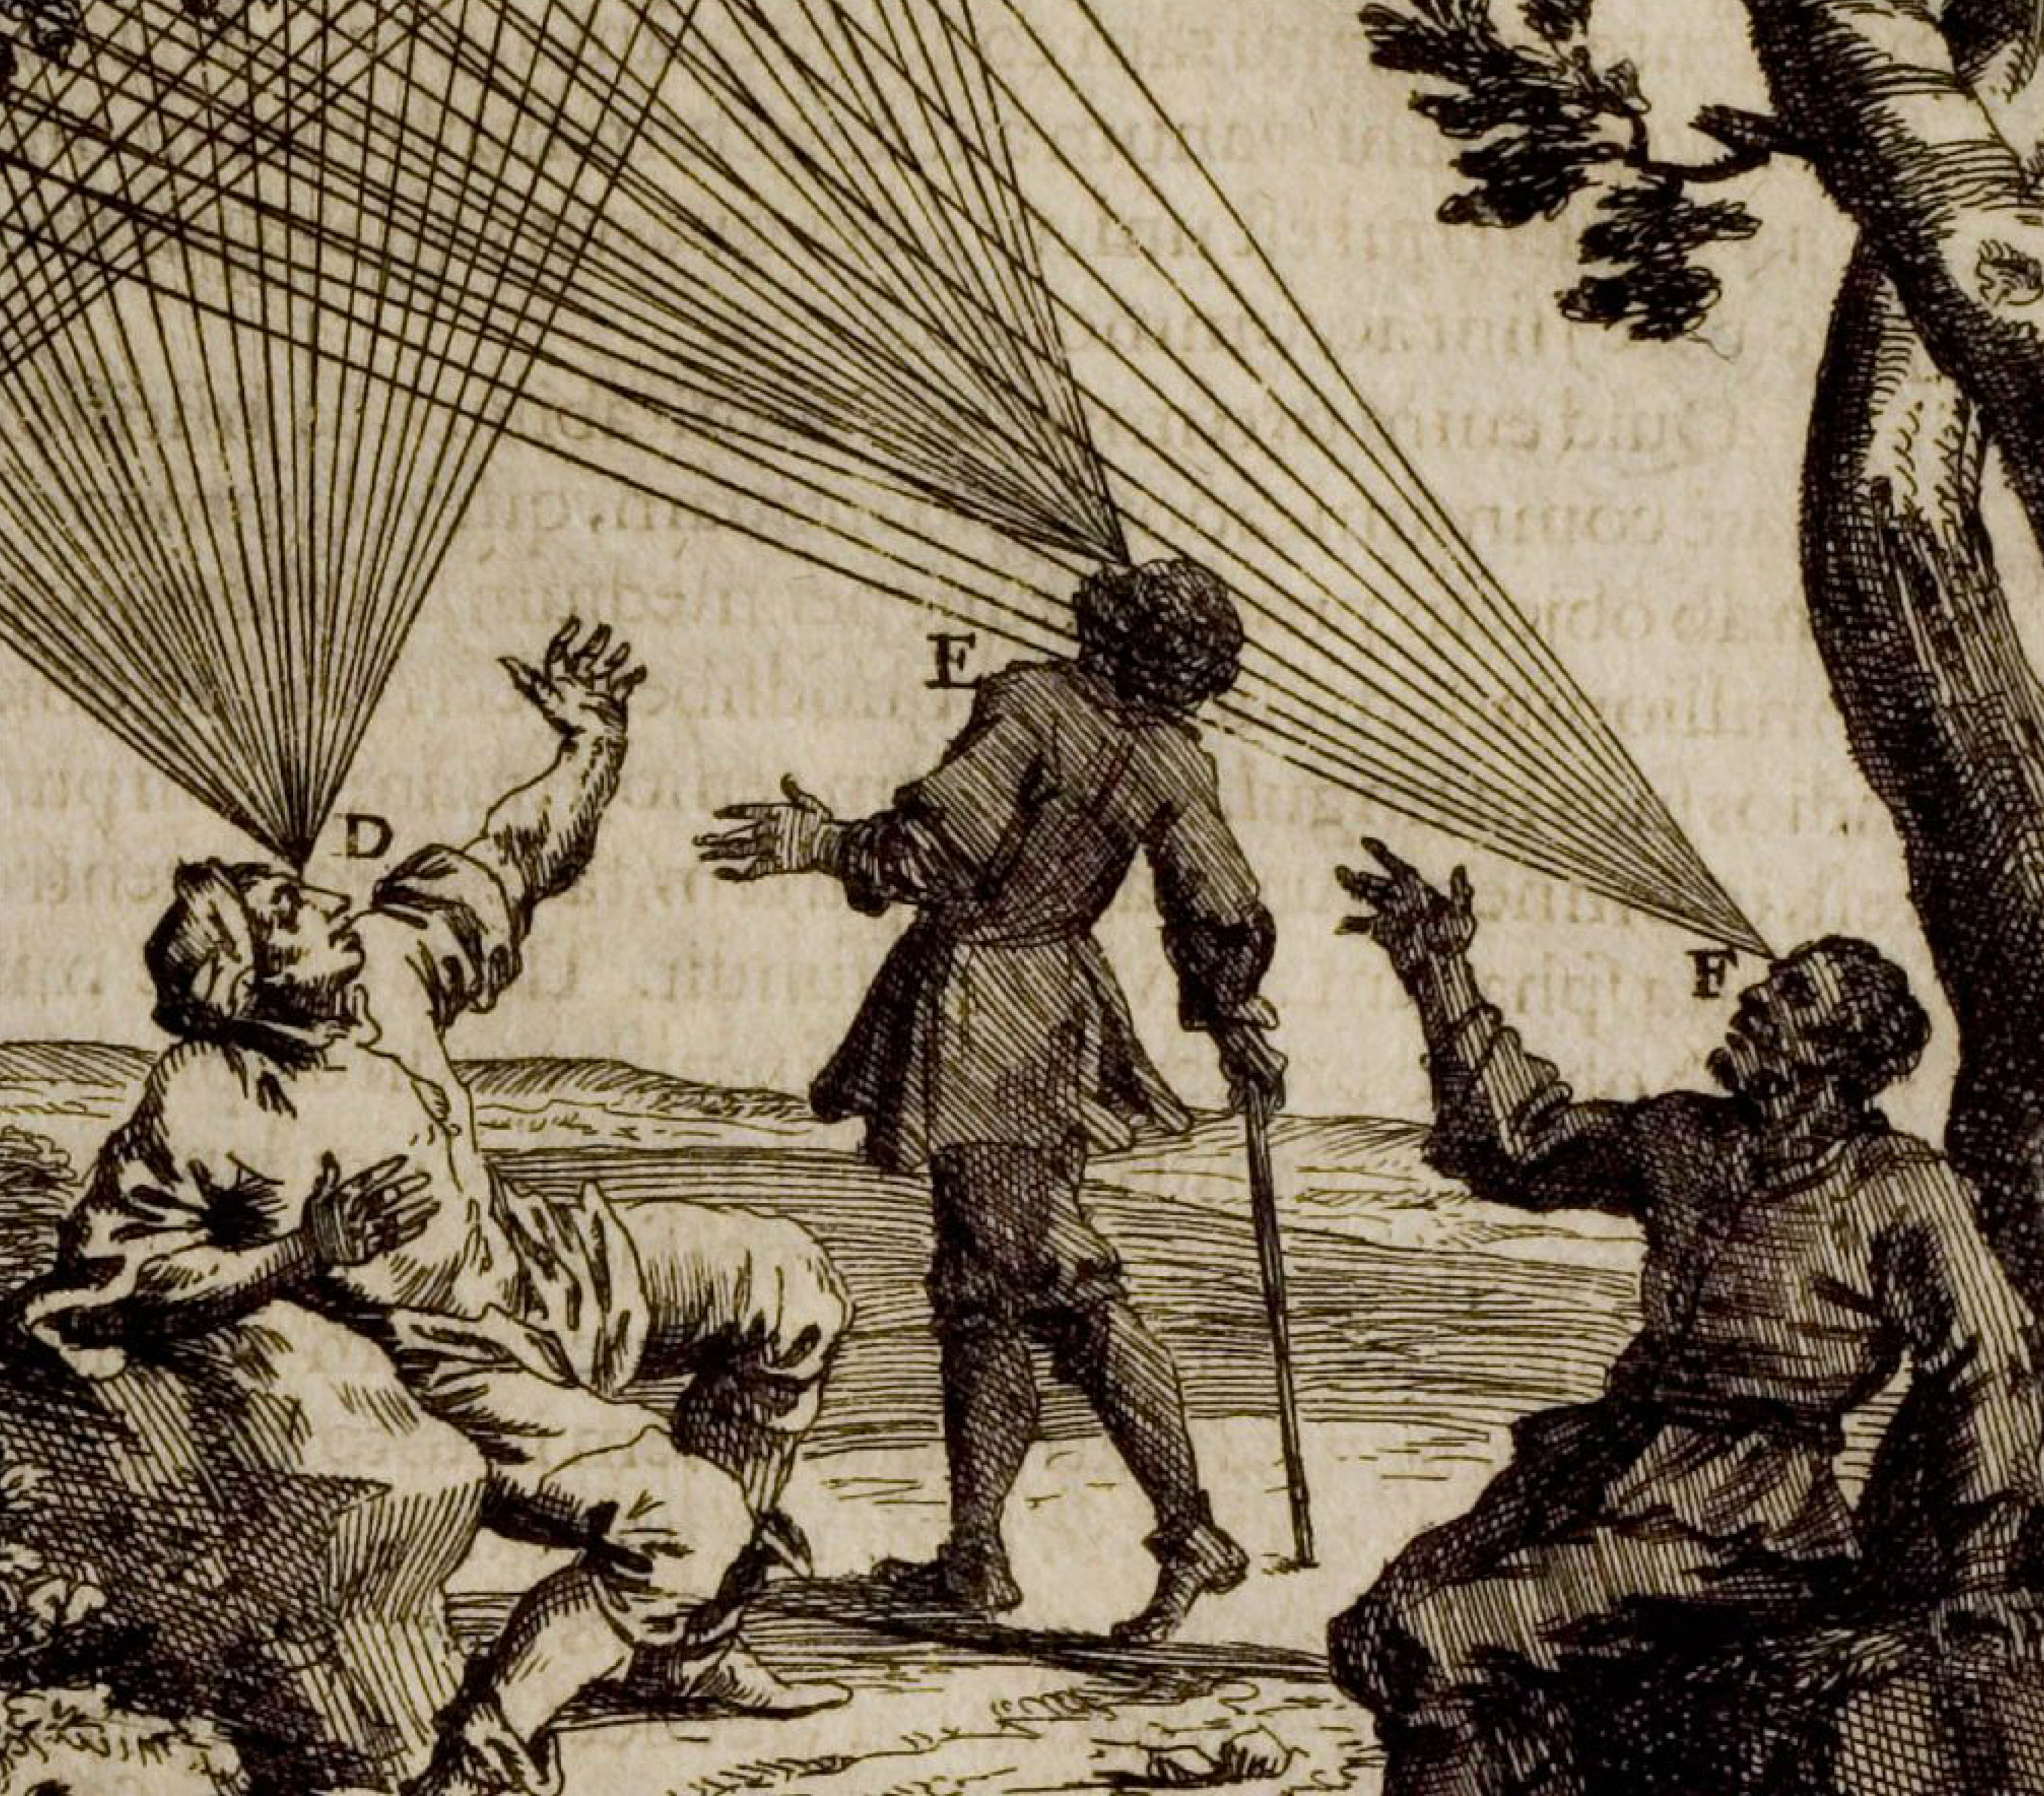
\includegraphics[width= 1\linewidth]{1}
		\vspace*{-10pt}
	\end{figure}
	Khi các nhà toán học Jeff Kahn và Gil Kalai lần đầu tiên đưa ra giả thuyết ``ngưỡng kỳ vọng" năm $2006$, chính họ không tin vào nó. Phát biểu của họ -- một khẳng định rộng về các đối tượng toán học gọi là các đồ thị ngẫu nhiên -- trông có vẻ quá mạnh, quá bao quát, quá táo bạo để có thể là đúng. Tưởng chừng như đó là suy nghĩ mơ mộng hơn là một chiêm nghiệm về sự thật toán học. Ngay cả như thế, chưa ai có thể chỉ ra nó sai, và giả thuyết đã nhanh chóng trở thành một trong những bài toán mở quan trọng nhất trong lĩnh vực.
	\vskip 0.1cm
	Giờ đây, hơn $15$ năm sau, hai nhà toán học trẻ ở Đại học Stanford (Stanford University) đã làm điều mà Kahn và Kalai cho rằng không thể: trong một tiền ấn phẩm ngắn đến ngạc nhiên đăng trên Internet mới chỉ một vài tuần trước, Jinyoung Park và Phạm Tuấn Huy đã đưa ra một chứng minh đầy đủ cho giả thuyết này.
	\vskip 0.1cm
	``Nó đơn giản và mới mẻ đến  kinh ngạc," Kalai nói. ``Nó kỳ thú. Nó tuyệt vời."
	\vskip 0.1cm
	Kết quả trên tự động chứng tỏ hàng trăm các phát biểu riêng biệt khác, mà mỗi phát biểu này đều rất khó để chứng minh -- và nó có cả những hệ quả sâu hơn cho hiểu biết của chúng ta về các đồ thị ngẫu nhiên và, tổng quát hơn, các tập hợp trong toán học.
	\vskip 0.1cm
	``Tôi gọi chứng minh của họ là ảo diệu,"  Jacob Fox -- một nhà toán học ở Stanford, đồng thời là thầy hướng dẫn PhD của Tuấn Huy -- nói. `` Đây sẽ là một phần chính của lĩnh vực trong tương lai."
	\vskip 0.1cm
	\textbf{\color{duongvaotoanhoc}Đóng băng một đồ thị}
	\vskip 0.1cm
	Giả thuyết Kahn--Kalai rất rộng -- nó được viết theo ngôn ngữ trừu tượng của các tập hợp và các phần tử của chúng -- nhưng nó có thể được hiểu bằng cách xét một trường hợp đơn giản. Đầu tiên, tưởng tượng một đồ thị: một tập hợp các điểm, hoặc đỉnh, nối với nhau bởi các đường, hay cạnh. Để làm đồ thị trở nên ngẫu nhiên, lấy một đồng xu không cân đối -- đồng xu này lật ngửa với xác suất $1\%$, hay $30\%$, hay bất kỳ xác suất nào từ $0\%$ đến $100\%$ -- và tung nó một lần với mỗi cặp đỉnh. Nếu đồng xu lật ngửa, nối cặp đỉnh này với một cạnh; nếu đồng xu lật sấp, không nối. Lặp lại quá trình này với mỗi cặp đỉnh \linebreak  có thể.
	\begin{figure}[H]
		\vspace*{-5pt}
		\centering
		\captionsetup{labelformat= empty, justification=centering}
		\includegraphics[width= 1\linewidth]{2}
		\caption{\small\textit{\color{duongvaotoanhoc}Nhà toán học Jinyoung Park, Đại học Stanford.}}
		\vspace*{-10pt}
	\end{figure}
	Các nhà toán học muốn biết khi nào một đồ thị như thế có thể chứa một cấu trúc thú vị nào đó. Có thể nó chứa một tam giác. Hoặc có thể nó chứa một chu trình Hamilton, một chuỗi các cạnh khép kín đi qua mỗi đỉnh đúng một lần. Ta có thể nghĩ về bất kỳ thuộc tính nào, miễn là nó ``tăng" -- nghĩa là nếu ta bổ sung thêm các cạnh vào một đồ thị đã có thuộc tính đó thì ta sẽ không phá hỏng thuộc tính đó.
	\vskip 0.1cm
	Nếu xác suất đồng xu lật ngửa là thấp, thì các cạnh sẽ hiếm, và các thuộc tính như các chu trình Hamilton có vẻ sẽ không xuất hiện. Nhưng nếu bạn làm tăng xác suất, một điều kỳ lạ sẽ xảy ra. Mỗi thuộc tính có một thứ gọi là ngưỡng: một xác suất mà khi đó cấu trúc hiện ra, thường rất đột ngột. Cũng giống như những tinh thể nước đá tạo thành khi nhiệt độ hạ xuống dưới $0$ độ Celsius, sự xuất hiện đột nhiên của một thuộc tính cụ thể trở nên cực kỳ giống như nhiều cạnh được bổ sung vào đồ thị. Khi các cạnh được thêm vào một đồ thị ngẫu nhiên có $N$ đỉnh với xác suất nhỏ hơn $\log(N)/N$, ví dụ, đồ thị có lẽ không chứa một chu trình Hamilton nào. Nhưng khi xác suất được điều chỉnh nhỉnh hơn $\log(N)/N$ chỉ một sợi tóc, một chu trình Hamilton trở nên cực kỳ có thể.
	\vskip 0.1cm
	Các nhà toán học muốn xác định các ngưỡng này cho nhiều thuộc tính đáng quan tâm. ``Các ngưỡng có lẽ là điều cơ bản nhất bạn muốn hiểu," Fox nói. ``Tôi nhìn một đối tượng ngẫu nhiên; nó có thuộc tính mà tôi quan tâm không?" Trong khi ngưỡng đã được tính cho các chu trình Hamilton và một vài cấu trúc riêng biệt khác, trong  hầu hết các trường hợp, việc xác định một ngưỡng chính xác, hoặc ngay cả một ước lượng tốt cho ngưỡng, cũng là rất khó.
	\vskip 0.1cm
	Vì thế các nhà toán học thường dựa trên một tính toán dễ hơn, nhằm đưa ra một giá trị nhỏ nhất có thể, hoặc một chặn dưới, cho ngưỡng này. ``Ngưỡng kỳ vọng" này được tính chủ yếu bằng các lấy một trung bình có trọng số. ``Cái hay về ngưỡng kỳ vọng này là nó rất dễ tính," David Conlon -- một nhà toán học tại Viện Công nghệ California (California Institute of Technology) -- nói. ``Nói nôm na, bạn có thể tính ngưỡng kỳ vọng này chỉ trong hai dòng cho hầu như bất kỳ thứ gì."
	\vskip 0.1cm
	Nhưng các trung bình có thể đánh lừa. Ví dụ, với các chu trình Hamilton, ngưỡng kỳ vọng là  $1/N$, thấp hơn giá trị thực $\log(N)/N$ bởi một thừa số $\log(N)$.
	\vskip 0.1cm
	Năm $2006$, Kahn và Kalai cho rằng đây có thể là tình huống xấu nhất. Giả thuyết mang tên của họ phát biểu rằng khoảng cách giữa ngưỡng kỳ vọng và ngưỡng thực tế không bao giờ lớn hơn một thừa số lô--ga--rít. Giả thuyết này, theo Conlon, ``về bản chất lấy câu hỏi trọng tâm về các đồ thị ngẫu nhiên và đưa ra một câu trả lời tổng quát cho nó."
	\vskip 0.1cm
	Nhưng đó chỉ là một trường hợp đơn giản. Giả thuyết liên quan tới nhiều đồ thị ngẫu nhiên hơn. Nếu đúng, nó cũng đúng cho các dãy số ngẫu nhiên, cho các tổng quát hoá của các đồ thị gọi là các siêu đồ thị, và ngay cả những kiểu hệ thống rộng hơn. Đó là vì Kahn và Kalai viết phát biểu của họ dưới dạng các tập hợp trừu tượng. Các đồ thị ngẫu nhiên đóng vai trò một trường hợp riêng biệt -- một đồ thị ngẫu nhiên có thể xem như một tập con ngẫu nhiên của tập hợp tất cả các cạnh -- nhưng có nhiều đối tượng khác cũng nằm trong phạm vi của giả thuyết. ``Thật lạ lùng, khi bạn đang làm việc với các đồ thị, chứng minh nó trong ngữ cảnh đó là rất khó," Conlon nói. ``Nhưng một cách nào đó, nhảy sang ngữ cảnh trừu tượng này làm lộ ra cái rốn của nó."
		\begin{figure}[H]
		\vspace*{-5pt}
		\centering
		\captionsetup{labelformat= empty, justification=centering}
		\includegraphics[width= 1\linewidth]{3}
		\caption{\small\textit{\color{duongvaotoanhoc}Nhà toán học Gil Kalai, Đại học Hebrew ở Jerusalem.}}
		\vspace*{-15pt}
	\end{figure}
	Chính mức tổng quát này khiến phát biểu dường như không thể tin được. ``Đó là một giả thuyết rất dũng cảm," Shachar Lovett -- một nhà khoa học máy tính ở Đại học California, San Diego (University of California, San Diego) -- nói. Vì một lẽ, nó sẽ ngay lập tức đơn giản hóa một nỗ lực to lớn trong tổ hợp -- cố gắng tính các ngưỡng cho các thuộc tính khác nhau. ``Các câu hỏi dường như cần những chứng minh rất dài và phức tạp đột ngột biến mất ngay," Alan Frieze -- một nhà toán học tại Đại học Carnegie Mellon (Carnegie Mellon University) -- nói. ``Các chứng minh trở thành các hệ quả tầm thường của giả thuyết này."
	\vskip 0.1cm
	Việc nhiều bài toán có vẻ không liên quan có thể được giải quyết bằng một giả thuyết rộng như thế  có vẻ như quá mức  đối với nhiều nhà toán học. ``Nói thật, nó có vẻ hoàn toàn điên rồ," Conlon nói. Sau khi tạo ra giả thuyết này, Kahn và Kalai đã không cố gắng chứng minh nó. Họ đã nghiên cứu nhằm tìm ra phản ví dụ. Có rất nhiều ngữ cảnh để khám phá, họ nghĩ rằng thế nào họ cũng gặp được một cái [phản ví dụ].
	\vskip 0.1cm
	Nhưng hóa ra, ``câu chuyện tiến triển theo một cách rất khác" so với họ mong đợi, Kalai nói.
	\vskip 0.1cm
	\textbf{\color{duongvaotoanhoc}Con đường hoa hướng dương}
	\vskip 0.1cm
	Các phương pháp mà sau này sẽ dẫn đến một chứng minh mới cho giả thuyết Kahn--Kalai bắt đầu với một đột phá trong một bài toán khác tưởng chừng chẳng liên quan. Theo nhiều cách, câu chuyện bắt đầu với giả thuyết hoa hướng dương, một câu hỏi đưa ra bởi các nhà toán học Paul Erdős và Richard Rado năm $1960$. Giả thuyết hoa hướng dương xem xét rằng liệu các bộ tập hợp (collections of sets) có thể được xây dựng theo cách giống như các cánh hoa hướng dương hay không.
	\vskip 0.1cm
	Năm $2019$, Lovett là thành viên của một nhóm nghiên cứu đã tiến rất gần tới một lời giải hoàn chỉnh của bài toán hoa hướng dương. Tại thời điểm đấy, công trình đó tưởng chừng hoàn toàn tách biệt với giả thuyết Kahn--Kalai, vốn dùng đến xác suất. ``Tôi không thấy bất kỳ kết nối nào với giả thuyết của chúng tôi," Kalai nói. Lovett cũng thế, ông nói rằng ``chúng tôi không hề biết về những câu hỏi đấy. Chúng tôi quan tâm tới các hoa hướng dương."
	Nhưng Kahn, Park (nghiên cứu sinh tiến sĩ của Kahn tại thời điểm đó) và các đồng nghiệp đã liên kết hai giả thuyết khi họ cố gắng chứng minh một phiên bản lỏng hơn của giả thuyết Kahn--Kalai một vài tháng sau đó. (Chứng minh của họ đã được công bố trên tạp chí \textit{ Annals of Mathematics} năm $2021$.) Giả thuyết yếu hơn này, phát biểu bởi nhà toán học Pháp Michel Talagrand, thay ngưỡng kỳ vọng Kahn--Kalai bởi một ngưỡng kỳ vọng ``phân số" -- về bản chất là một cách khác để lấy trung bình có trọng số. Định nghĩa mới này ``cho bạn thêm không gian để làm việc," Lovett nói.
	\vskip 0.1cm
	Nhóm của Kahn và Park nhận thấy rằng họ có thể trích xuất các kỹ thuật từ kết quả hoa hướng dương năm $2019$, tinh chỉnh chúng, và áp dụng vào giả thuyết Talagrand. ``Đây chắc chắn là cái khiến chúng tôi bắt đầu," Kahn nói.
	\vskip 0.1cm
	Các nhà toán học dùng một cách tiếp cận vòng lặp cho bài toán.  Mục tiêu của họ là chứng tỏ rằng  nếu họ chọn một tập hợp ngẫu nhiên -- ví dụ một đồ thị ngẫu nhiên -- nó có thể chứa một cấu trúc ví dụ như một chu trình Hamilton. Nhưng thay vì chọn toàn bộ một tập hợp ngẫu nhiên ngay một lúc, họ chọn nó theo từng phần, một quá trình tương tự như cách mà Lovett và các đồng nghiệp tiếp cận giả thuyết hoa hướng dương. ``Chúng tôi thực hiện lặp lại một loại quá trình ngẫu nhiên," Park nói. ``Chúng tôi chọn một vài cạnh theo từng bước" cho tới khi chúng chứa đựng toàn bộ một chu trình Hamilton.
	\vskip 0.1cm
	Để làm điều này, nhóm nghiên cứu sử dụng một khái niệm về ngẫu nhiên gọi là trải. Nếu các chu trình Hamilton ``trải ra"  một cách đẹp đẽ, nghĩa là không quá nhiều chu trình chứa cùng một cạnh hay một tập con các cạnh. ``Một cách nào đó, bộ các tập hợp trải ra đẹp trong không gian," Tuấn Huy nói. ``Nó không quá co cụm hoặc tập trung trên bất kỳ phần nào." Nếu các chu trình được phân bố tốt theo cách này, nó đảm bảo rằng quá trình lấy ngẫu nhiên theo từng phần -- ngay cả khi nó thất bại cho nhiều chu trình Hamilton -- sẽ tạo được thành công ít nhất một chu trình [Hamilton].
	\vskip 0.1cm
	Cách tiếp cận này là khả thi nhờ một tương đương quan trọng:  sự trải có thể được định lượng theo một cách liên quan trực tiếp tới ngưỡng kỳ vọng phân số. Vì điều này, các nhà toán học có thể viết lại giả thuyết Talagrand dưới dạng trải.
	\vskip 0.1cm
	Thú vị làm sao, chứng minh của giả thuyết yếu hơn này đủ để giải quyết một loạt các bài toán liên quan tới ngưỡng. ``Mỗi hệ quả của giả thuyết đầy đủ mà chúng ta biết cũng là một hệ quả của giả thuyết yếu hơn," Kahn nói. Thực ra, với ông, Kalai và những người khác, điều này gợi ý rằng hai giả thuyết có thể hầu như là giống nhau -- rằng các giá trị của các ngưỡng kỳ vọng phân số và ngưỡng kỳ vọng ban đầu về mặt cơ bản là bằng nhau. Nếu ai đó có thể chứng minh sự tương đương  này, họ sẽ chứng minh được giả thuyết Kahn--Kalai. ``Tôi đã luôn nghĩ rằng cách duy nhất để chứng minh giả thuyết của chúng tôi là chứng minh điều này," Kahn nói.
	\vskip 0.1cm
	Nhưng đó không phải là điều đã xảy ra. Trong khi các nhà toán học khác cố gắng đi theo hướng này để chứng minh hoàn toàn giả thuyết Kahn--Kalai, Park và Tuấn Huy tìm ra một cách tiếp cận hoàn toàn mới. ``Jinyoung và Tuấn Huy tìm thấy một lập luận trực tiếp đến kinh ngạc, ngắn đến kinh ngạc, xuyên qua tất cả những thứ đó," Conlon nói. ``Thật là phi thường. Tôi không hề trông đợi điều này."
	\vskip 0.1cm
	Kahn đồng ý. ``Đây là một trong những điều đẹp đẽ trong toán học," ông nói.
	``Những thứ mà mọi người nghĩ rằng vô vọng thực ra lại không chỉ không vô vọng, mà còn chẳng khó nữa."
	\vskip 0.1cm
	\textbf{\color{duongvaotoanhoc}Một tiếp cận bất ngờ}
	\vskip 0.1cm
	Thoạt tiên, cả Park và Tuấn Huy đều không có ý định tấn công giả thuyết ban đầu. Khi bắt đầu học về bài toán khi còn là nghiên cứu sinh, Park ``có thể cảm nhận vẻ đẹp và sức mạnh của giả thuyết này," cô nói. ``Nhưng tôi chưa bao giờ tưởng tượng ra rằng mình có thể chứng minh được nó."
	\vskip 0.1cm
	``Điều đó chẳng hề có trong tâm trí của chúng tôi," Tuấn Huy nói thêm.
	\vskip 0.1cm
	Thay vào đó, họ đang làm việc với một giả thuyết khác đưa ra bởi Talagrand khi họ bị ``đánh thức bởi một phép màu," Tuấn Huy nói. Họ nhận ra rằng ``bức tranh mà chúng ta có ở đây, các ý tưởng mà chúng ta có,  theo một cách nào đó, có vẻ nó mạnh hơn vẻ bề ngoài của nó." Các ý tưởng này, họ nghĩ, có thể đủ mạnh để đưa họ thẳng tới một chứng minh của bài toán Kahn--Kalai.
	\vskip 0.1cm
	Trong suốt một đêm không ngủ vào tháng Ba, họ đã tìm ra cách chứng minh.
	\vskip 0.1cm
	Không giống như ngưỡng kỳ vọng phân số, ngưỡng kỳ vọng thông thường không liên quan tới trải. Trải ``cho bạn một điểm khởi đầu. Và nếu bạn đi đến giả thuyết ban đầu, phiên bản không phân số, điểm khởi đầu ấy biến mất," Kahn nói. ``Vì thế nó có vẻ rất khó."
	\vskip 0.1cm
	``Thế bạn làm gì?" Tuấn Huy nói. ``Trong trường hợp này, chúng tôi thay đổi góc nhìn của mình."
	\vskip 0.1cm
	Cụ thể hơn, họ nghĩ về bài toán  theo ngôn ngữ của  một đối tượng toán học gọi là một phủ. Một phủ là một bộ các tập hợp, mà mỗi đối tượng với một thuộc tính nào đó chứa một trong các tập hợp này. Ví dụ, một phủ của mọi chu trình Hamilton là bộ tất cả các cạnh. Mọi chu trình Hamilton sẽ chứa một trong các cạnh này.
	\vskip 0.1cm
	Park và Tuấn Huy viết lại giả thuyết Kahn--Kalai theo một cách cho phép họ  sử dụng các phủ. Giả thuyết ban đầu đưa ra ràng buộc về xác suất ngửa của đồng xu để  đảm bảo một đồ thị hay tập hợp ngẫu nhiên  có một thuộc tính nào đó. Cụ thể, nó nói rằng xác suất phải ít nhất bằng ngưỡng kỳ vọng cho thuộc tính nhân với một thừa số lô--ga--rít. Park và Tuấn Huy xoay ngược vấn đề lại: Nếu một thuộc tính ít khả năng  xuất hiện, thì xác suất gắn với đồng xu  thấp hơn ngưỡng kỳ vọng nhân với một thừa số lô--ga--rít.
	\begin{figure}[H]
		\vspace*{-5pt}
		\centering
		\captionsetup{labelformat= empty, justification=centering}
		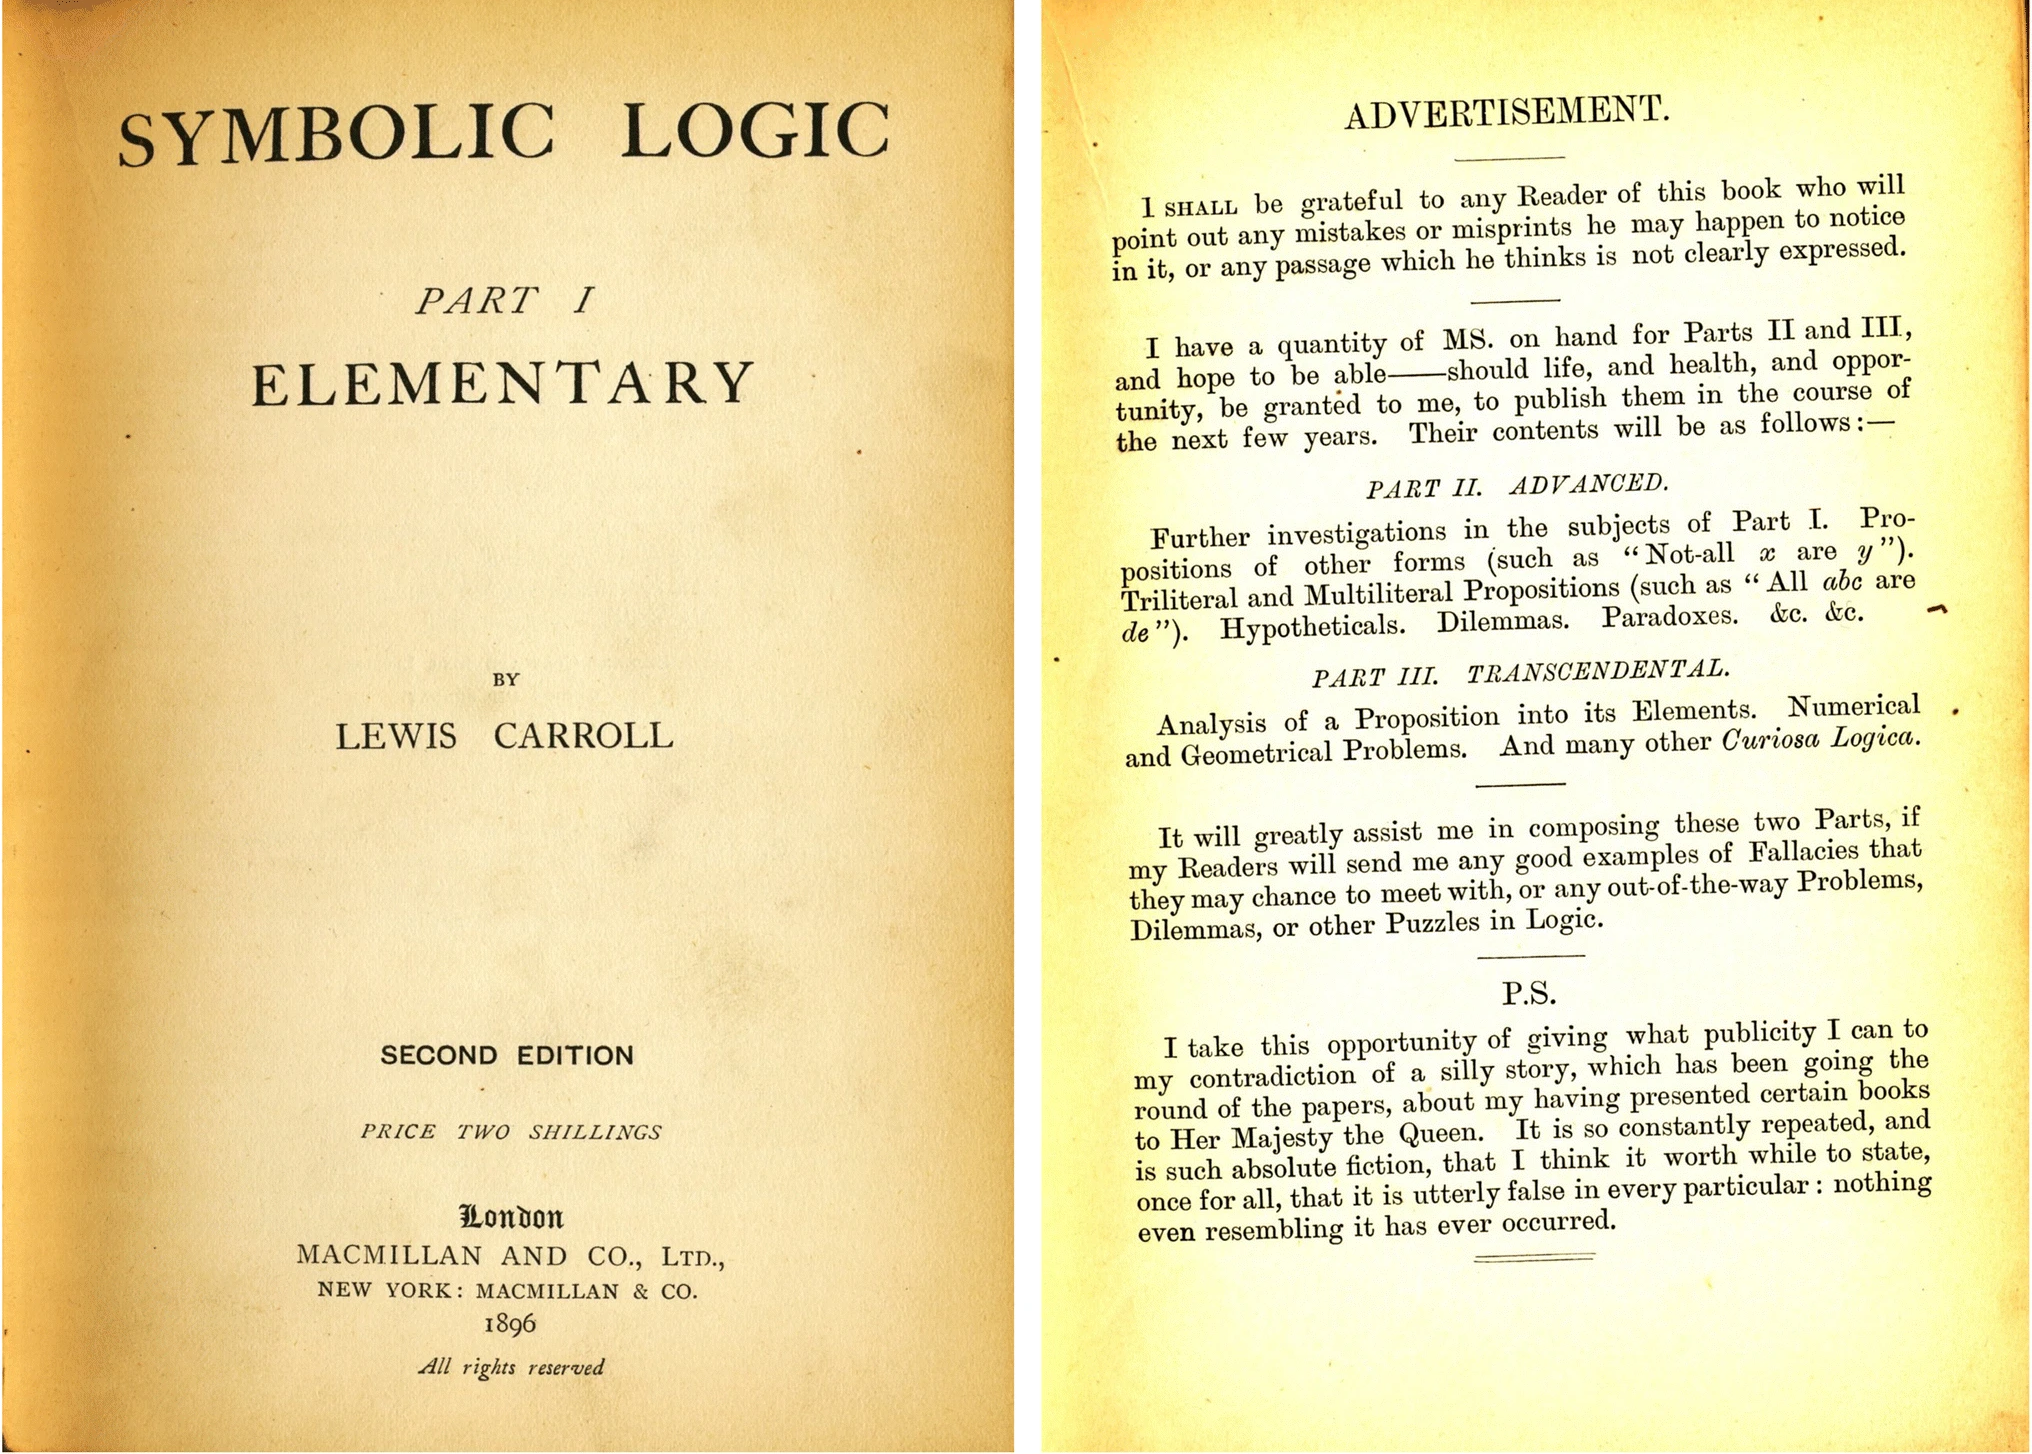
\includegraphics[width= 1\linewidth]{4}
		\caption{\small\textit{\color{duongvaotoanhoc}Nhà toán học Phạm Tuấn Huy, Đại học Stanford.}}
		\vspace*{-10pt}
	\end{figure}
	Đó là nơi mà các phủ xuất hiện: Khi một phủ nhỏ có thể được xây dựng cho một tập con các cấu trúc (như một bộ các chu trình Hamilton), nghĩa là đóng góp của tập hợp con đó  vào ngưỡng kỳ vọng là nhỏ. (Nhớ rằng ngưỡng kỳ vọng được tính bằng cách lấy một loại trung bình có trọng số trên mọi cấu trúc có thể có một dạng cho trước.) Vì thế điều mà Park và Tuấn Huy cần chứng minh là nếu một tập hợp ngẫu nhiên ít khả năng chứa cấu trúc được quan tâm, phải tồn tại một phủ nhỏ cho mọi cấu trúc như vậy. Phần chính trong chứng minh của họ dành cho việc xây dựng phủ nhỏ ấy.
	\vskip 0.1cm
	Họ làm điều này bằng cách sử dụng một quá trình lấy mẫu theo từng phần tương tự như cái mà họ đã dùng trong các kết quả trước, đồng thời giới thiệu cái mà Fox gọi là ``một lập luận đếm rất thông minh." Một tuần sau đêm tháng Ba không ngủ, họ đăng một bài báo đẹp $6$ trang lên mạng.
	\vskip 0.1cm
	``Chứng minh của họ là siêu đơn giản. Họ dùng ý tưởng cơ bản mà chúng tôi đã phát triển và [các ý tưởng khác từ] những bài báo kia và thêm một bước chuyển vào nó," Lovett nói. ``Và với bước chuyển mới này, mọi thứ một cách nào đó trở nên dễ hơn rất, rất nhiều."
	\vskip 0.1cm
	Frieze đồng ý. ``Tôi không thể giải thích, nhưng thật ngạc nhiên là nó đúng," ông nói.
	\vskip 0.1cm
	Cũng như kết quả phân số, giả thuyết Kahn--Kalai, giờ đây đã được chứng minh là đúng, tự động dẫn đến một loạt các giả thuyết liên quan. Nhưng hơn thế, ``đây là một kỹ thuật chứng minh mạnh có lẽ sẽ dẫn đến nhiều điều mới,"  Noga Alon -- nhà toán học tại Đại học Princeton (Princeton University) -- nói. ``Họ đã làm đúng cách."
	\vskip 0.1cm
	Park và Tuấn Huy đã bắt đầu áp dụng phương pháp của họ cho các bài toán khác. Họ đặc biệt quan tâm đến việc hiểu chính xác hơn khoảng cách giữa ngưỡng kỳ vọng và ngưỡng thực tế. Bằng cách chứng minh giả thuyết Kahn--Kalai, họ đã chỉ ra  rằng khoảng cách này không quá một thừa số lô--ga--rít  -- nhưng đôi khi khoảng cách này là nhỏ hơn, hoặc thậm chí không tồn tại. Hiện tại, không có một cơ chế rộng hơn để phân loại khi nào mỗi tình huống này có thể đúng; các nhà toán học phải tính ra theo từng trường hợp. Giờ đây, ``chúng tôi nghĩ rằng với kỹ thuật hiệu quả mà chúng tôi có, hy vọng chúng tôi  có thể xác định các ngưỡng này một cách chính xác hơn nhiều," Tuấn Huy nói.
	\vskip 0.1cm
	Và chứng minh của họ có thể có các hệ quả khác nữa. ``Giả thuyết Kahn--Kalai  hoàn toàn chưa phải  là kết thúc của câu chuyện," Park nói.
	\vskip 0.2cm
	\PIbox{Viện Toán học Clay (Clay Mathematics Institute) thông báo rằng Phạm Tuấn Huy đã được trao tặng Học bổng Nghiên cứu Clay (Clay Research Fellowship) năm $2023$. Phạm Tuấn Huy sẽ nhận bằng tiến sĩ từ Đại học Stanford năm $2023$, dưới sự hướng dẫn của Jacob Fox. Anh cũng được bổ nhiệm làm một Nghiên cứu viên Clay (Clay Research Fellow) trong $5$ năm bắt đầu từ $01/07/2023$.
		\vskip 0.1cm
		Tiêu chí tuyển chọn chính của các Nghiên cứu viên Clay là chất lượng nghiên cứu vượt trội của ứng cử viên và lời hứa của ứng cử viên là sẽ trở thành một nhà toán học hàng đầu. Các Nghiên cứu viên Clay được tuyển dụng bởi Viện Toán học Clay, nhưng có thể làm việc ở bất kỳ nơi nào tại Mỹ, Châu Âu, hay một nơi khác trên thế giới.
		\vskip 0.1cm
		Các Nghiên cứu viên Clay trước đây đã trở thành những nhà toán học hàng đầu, trong đó có nhiều nhà toán học được trao tặng Huy chương Fields như Akshay Venkatesh ($2018$), Artur Avila ($2014$), Elon Lindenstrauss ($2010$), Manjul Bhargava ($2014$), Maryam Mirzakhani ($2014$), Terence Tao ($2006$), June Huh ($2022$), James Maynard ($2022$), Peter Scholze ($2018$). Giáo sư Ngô Bảo Châu (Huy chương Fields $2010$) được trao tặng Giải thưởng Nghiên cứu Clay (Clay Research Award) năm $2004$.}
\end{multicols}